% !TeX program = lualatex
% !TeX root = main.tex
\renewcommand*{\dictumwidth}{0.5\textwidth}
\setchapterpreamble[u]{%
	\dictum[Verity Stob%\footnotemark
]{``The primary duty of an exception handler is to get the error out of the lap of the programmer and into the surprised face of the user.''}}
\chapter{Implementation}
\label{chap:implementation}
\bigskip
\textit{After seeing the needed interfaces in the last chapter, there will be a description about the overall software environment and which components had to be modified in order to implement the processor P- and C-state tracing.}
%\footnotetext{\url{http://www.regdeveloper.co.uk/2006/01/11/exception_handling/page2.html}}

\bigskip
\lettrine[lines=2, lhang=.1, lraise=.1]{T}{he} extended programs are parts of a whole software environment developed at the ``Research Group Parallel and Distributed Systems'' (PVS). The projects intend to create and visualize trace files. A trace file is the record of the actions a program does respectively how it interacts with its environment.

The \emph{ResourcesUtilizationTracingLibrary} captures the component utilization from the OS, for example the used RAM or the transfer rates of the NIC, whereas the \emph{PowerTracingLibrary} uses an external power meter to record the power consumption of the node. The \emph{HDMPIwrapper} keeps track of MPI calls and utilizes the \emph{Trace Writing Library} to actually write the traces to the hard drive. These projects are running while the observed MPI program runs, meaning they have some performance impact and are therefore implemented in the programming language C. The performance influence differs between 0.60\,\% (500\,ms) and 10.34\,\% (20\,ms)\cite{krempel} and is mainly based on the interval length the tracing library is waiting until it records a new trace point.

Additionally, there exist projects written in Java in order to evaluate the trace files. \emph{HDTraceFormat} is used to read and modify trace files and \emph{Sunshot} can visualize them. \emph{HDPowerEstimation} can calculate the consumed energy and is able to estimate power savings based on different reschedule strategies. This shows the potential effect of activating power saving mechanisms in a cluster. HDPowerEstimation provides computed savings and pre-after-power curves.

ResourcesUtilzationLibrary will be able to trace P- and C-states, a power estimator---in the future merged into HDPowerEstimation---will be able to read these states and use them, exampled in a new strategy.

\newpage
\noindent
Figure \ref{fig:wrapper} depicts the software environment and how the described components are interacting with each other.

%
\begin{figure}[h!]
	\centering
%	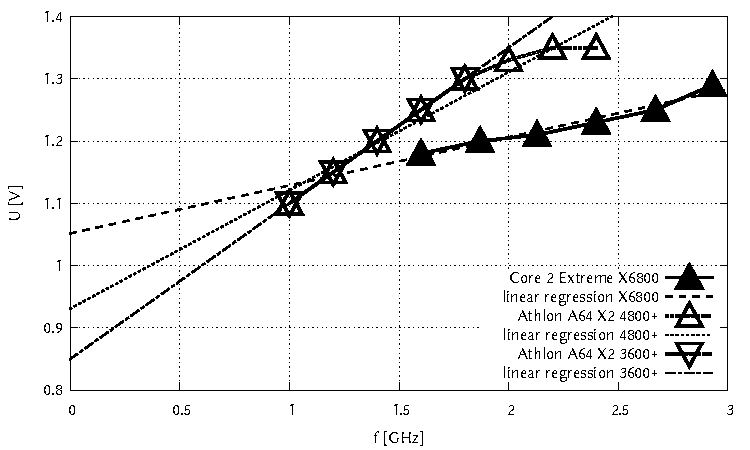
\includegraphics[width=\linewidth]{pix/pstates/pstates}
	% !TeX program = lualatex
% !TeX root = ../../main.tex
\begin{tikzpicture}
\draw 	(0,-1em) node[inner sep=5pt, minimum width=15em, minimum height=2em, draw] (PM) {Power Meter}

		(-6em,4em) node[rectangle split, rectangle split parts=2, inner sep=5pt,draw] (N1) {OS \nodepart{second} Node}
		(-2em,4em) node[rectangle split, rectangle split parts=2, inner sep=5pt,draw] (N2) {OS \nodepart{second} Node}
		(2em,4em) node[rectangle split, rectangle split parts=2, inner sep=5pt,draw] (N3) {OS \nodepart{second} Node}
		(6em,4em) node[rectangle split, rectangle split parts=2, inner sep=5pt,draw] (N4) {OS \nodepart{second} Node}

		(0,14.5em) node[inner sep=5pt, minimum width=29em, minimum height=10em, draw] (W) {Wrapper}

		(0,11.5em) node[inner sep=5pt, minimum width=15em, minimum height=2em, draw] (PMP) {Parallel MPI Program}
		(0,17.5em) node[inner sep=5pt, minimum width=15em, minimum height=2em, draw] (TWL) {Trace Writing Library}
		(-9em,14.5em) node[inner sep=5pt, minimum height=2em, text width=8em, draw] (PTL) {Power Tracing Library}
		(9em,14.5em) node[inner sep=5pt, minimum height=2em, text width=9em, draw] (RUTL) {Resources Utilization Tracing Library}

		(0,21.5em) node[inner sep=5pt, minimum width=4, minimum height=2em, draw] (TF) {Trace Files}

%		(11.5em,21.5em) node[inner sep=5pt, minimum width=4, minimum height=2em, draw] (XF) {XML File}

		(0,25em) node[inner sep=5pt, minimum width=4, minimum height=2em, draw] (HDTF) {HDTraceFormat}

		(11.5em,29em) node[inner sep=5pt, minimum width=4, minimum height=2em, draw] (HDPE) {HDPowerEstimation}
		
%		(-11.5em,29em) node[inner sep=5pt, minimum width=6em, minimum height=2em, draw] (JFC) {JFreeChart}

		(-11.5em,25em) node[inner sep=5pt, minimum width=6em, minimum height=2em, draw] (HDJ) {Sunshot}

;
		\draw[<-, line width=1.3pt] (-6em,0em) -- (N1);
		\draw[<-, line width=1.3pt] (-2em, 0em) -- (N2);
		\draw[<-, line width=1.3pt] (2em, 0em) -- (N3);
		\draw[<-, line width=1.3pt] (6em, 0em) -- (N4);

		\draw[<->, line width=1.3pt] (-6em, 9.5em) -- (N1);
		\draw[<->, line width=1.3pt] (-2em, 9.5em) -- (N2);
		\draw[<->, line width=1.3pt] (2em, 9.5em) -- (N3);
		\draw[<->, line width=1.3pt] (6em, 9.5em) -- (N4);

		\draw[line width=2.2pt, line join=miter] (-7.35em, 5.5em) -- (-7.35em, 7.5em) -- (-7em, 7.5em);
		\draw[->, line width=2.2pt] (-7.35em, 7.5em) -| (RUTL);
		\draw[line width=2.2pt] (-3.35em, 7.5em) -- (-3.35em, 5.5em);
		\draw[line width=2.2pt] (0.65em, 7.5em) -- (0.65em, 5.5em);
		\draw[line width=2.2pt] (4.65em, 7.5em) -- (4.65em, 5.5em);

		\draw[->, line width=2.2pt] (PM) -| (PTL);
		\draw[->, line width=1.3pt] (TWL) -- (TF);
		\draw[<->, line width=1.3pt] (TF) -- (HDTF);
		\draw[<-, line width=1.3pt] (HDTF) |- (HDPE) node[midway, above, pos=0.8, text width=10em, font=\fontsize{10}{11}\selectfont] {Component Estimated Energy Consumption};
		\draw[->, line width=1.3pt] (HDTF) -| (HDPE) node[midway, above left, text width=6em, font=\fontsize{10}{11}\selectfont] {Node Energy Consumption};
%		\draw[dotted, line width=1.3pt] (XF) -- (HDPE) node[midway, below right, text width=6em, font=\fontsize{10}{11}\selectfont] {Component Utilization};

%		\draw[dotted, <-, line width=1.3pt] (JFC) -- (HDPE) node[midway, above, pos=0.8, text width=10em, font=\fontsize{10}{11}\selectfont] {Component Estimated Energy Consumption};
		\draw[<-, line width=1.3pt] (HDJ) -- (HDTF);
\end{tikzpicture}
\newcommand*\Captiontext{Tracing environment at the PVS cluster}
	\caption[\Captiontext]{\Captiontext\cite{minartz}}
	\label{fig:wrapper}
\end{figure}
%

%


\section{ResourcesUtilizationTracingLibrary}
\label{sec:rutl}
The basic workflow of the library consists of an initialization phase and the tracing phase. In the initialization phase, it checks which values should be traced based on the options marked in the \lstinline!struct rutSources_s! and then writes these values into the header of the trace file.
\newpage
\begin{lstlisting}[%
	language=C,%
	caption={Frequency tracing activated?},%
	%label={lst:freq},%
	numbers=left,%
	firstnumber=152]
if(!cpufreq_available()){
	tracingData->sources.CPU_FREQ_X = 0;
	INFOMSG("Could not find cpufreq!");}
if (tracingData->sources.CPU_FREQ_X){
	for (int i = 0; i < tracingData->staticData.cpu_num; ++i){
		ret = snprintf(strbuf, RUT_STRING_BUFFER_LENGTH, "CPU_FREQ_CPU%d", i);
		ADD_VALUE(group, strbuf, INT64, "Hz", "CPU_FREQ");
}	}
\end{lstlisting}
%
\lstinline!cpufreq_available()! checks if the sysfs interface for CPUFreq is available. If not, frequency tracing will be deactivated and an info message posted. Otherwise a unique string for every CPU will be composed and added to the traced values, along with some information like the datatype \lstinline!INT64! and the unit \lstinline!"Hz"! (in contrast to \lstinline!"%"! for percentage).

The implementation for CPUIdle is analogue.

%\superpar
The tracing phase is similar, but instead of saying how the value is called and its type, the actual value is written. After every iteration, the library checks if it should stop or continue, and then waits for the length of the interval, until it begins to trace again.

The actual frequency tracing is easy, because CPUFreq offers a shared library implementing the basic functionality.
%
%\begin{lstlisting}[%
%	language=C,%
%	caption={Frequency tracing},%
%	label={lst:freq},%
%	numbers=left,%
%	firstnumber=565]
%if (tracingData->sources.CPU_FREQ_X){
%	for (int i = 0; i < tracingData->staticData.cpu_num; ++i){
%		valuei64 = (gint64) (cpufreq_get_freq_kernel(i));
%		WRITE_I64_VALUE(tracingData, valuei64);
%		DEBUGMSG("CPU_FREQ_%d = %d kHz", i, valuei64);
%}	}
%\end{lstlisting}
%
\lstinline!cpufreq_get_freq_kernel(unsigned int core)! returns the frequency of the given core. Voltage tracing is not yet implemented. This will be done based on IPMI. Because every frequency can be mapped to a corresponding voltage, frequency tracing is sufficient for evaluation. Voltages can be gathered by reading the processor manual or using software like k10ctl or c2ctl\footnote{\url{http://www.ztex.de/misc/}}.

CPUIdle does not (yet?) have a programming interface---there has to be done a little more than at frequency tracing. First step is to save the old C-state usage times and then get the new ones.

%
\begin{lstlisting}[%
	language=C,%
	caption={Idle tracing},%
	%label={lst:idle},%
	name=idle,
	numbers=left,%
	firstnumber=575]
if (tracingData->sources.CPU_IDLE_X){
	/* save old values */
		. . .
	/* get new values */
	get_c_state_times(
		tracingData->oldValues.c_states, 
		tracingData->staticData.cpu_num,
		tracingData->staticData.c_states_num);
\end{lstlisting}
%

\noindent
\lstinline!int get_c_state_times(unsigned long int *cstates, int cpu, int states)! is the function to get the C-states. It takes three arguments: the pointer to an array, where the times spend in the C-states are stored, and the number of cores and C-states. Basically, the function traverses the specific folders and files in the sysfs interface of CPUIdle and writes the values to the array\cite{powertop}.

Because the times the processors have spend in a state are total values since the last system start, the differences between formal and recent values are needed. Those differences are added together to get the times the cores have spend in idle (in microseconds).
\begin{align*}
	\text{\lstinline!idle_time!} &= \sum\limits_{n=1}^{\text{\lstinline!states!}} \text{time in } C_n
\end{align*}
The active time (C0) is simply the interval length (given in milliseconds) minus the the time spend in idle. There might be a small divergence, because of the precision of the function used to send the tracing thread to sleep while not tracing (``\lstinline!g_usleep()! may have limited precision, depending on hardware and operating system; don't rely on the exact length of the sleep\cite{glib}.''). 

The reason for not just taking the usage time of C0 as the active time is caused in the absence of regular updates for this variable, and these seldom updates are not representing active time. An explanation for this behaviour lays in the mode of operation of CPUIdle, as only the function responsible for sending cores to idle is updating the usage values.

%
%\begin{lstlisting}[%
%	language=C,%
%	%caption={Idle tracing},%
%	%label={lst:idle},%
%	name=idle,
%	numbers=left,%
%%	firstnumber=594
%]
%	/* difference */
%		. . .
%	/* calculating time spend in idle for every core */	
%	for (int i = 0; i < tracingData->staticData.cpu_num; ++i){
%		
%		/* total time in idle */
%			. . .		
%		/* time not in idle: easy, interval - time in idle, 
%		 * careful as time in idle is given in microsecs */
%		guint64 interval = (tracingData->interval) * 1000;
%		guint64 c0 = interval - total;
%		valuef = c0 / interval * 100.0;
%						
%		WRITE_FLOAT_VALUE(tracingData, valuef);
%		DEBUGMSG("CPU_IDLE_C%d_%d = %f%%", 0, i, valuef);
%				
%		for (int j = 1; j < tracingData->staticData.c_states_num; ++j){
%			valuef = c_states[i * tracingData->staticData.c_states_num + j] / interval * 100.0;
%					
%			WRITE_FLOAT_VALUE(tracingData, valuef);
%			DEBUGMSG("CPU_IDLE_C%d_%d = %f%%", j, i, valuef);
%}	}	}
%\end{lstlisting}

The written values are the percentages the core has spend in these states: 
\begin{align*}
\text{\lstinline!interval_length!} &= \text{\lstinline!tracingData->interval!} \cdot 1000\\
percentage\,Cn &=  \frac{\text{time in } Cn}{\text{\lstinline!interval_length!}} \cdot 100
\end{align*}

%
%
\section{Power Estimator}
The structure of the power estimator resembles CPUFreq\,/\,CPUIdle. One part is the representation of a CPU (driver), the other part is a estimation strategy (governor). The driver has to provide values like the available frequencies or the power usage in the different C-states. It also has to implement miscellaneous functions for getting and setting values, and the function \lstinline!double!\,\lstinline!getPower(int frequency, float[] c_usage)! which is used by the governor to get the recent power consumption. To read the trace files the power estimator uses HDTraceFormat.

In the provided implementation \lstinline!getPower()! uses the consumption model presented in this thesis, which is extended by the actual usage of the processor in the intervals.

%
\begin{align*}
P_{recent} &= \text{\lstinline!max_power!} \cdot \frac{frequency_{recent}}{\text{\lstinline!max_frequency!}} \cdot \frac{voltage_{recent}^2}{\text{\lstinline!max_voltage!}^2}
\end{align*}
%
%The usage of the actual utilization is based on the factor \lstinline!idle!, describing the consumption at 0\,\% utilization $P_{idle} = \text{\lstinline!max_power!} \cdot \text{\lstinline!idle!}$. The consumption at \lstinline!util!\,\% utilization is

%\begin{align*}
%P_{recent} &= P_{recent} \cdot (u + \text{\lstinline!idle!} - u \cdot \text{\lstinline!idle!})
%\end{align*}
%
\lstinline!c_usage! contains the usage of the different C-states in this interval in percent. The next step is to use this information and add the consumptions of the other C-states, stored in \lstinline!power_cstates! to finally get the power consumption in this step.

\begin{align*}
P_{recent} &= P_{recent} \cdot \text{\lstinline!c_usage[0]!}\\
P_{idle} &= \sum (\text{\lstinline!power_cstates[n]!} \cdot \text{\lstinline!c_usage[n]!})\\
P_{total} &= P_{recent} + P_{idle}
\end{align*}
%
The implemented governor now just multiplies each consumption with its interval length and accumulates all these consumptions. 

\begin{align*}
E_{total} = \sum\limits^{steps} (\text{\lstinline!getPower()!} \cdot \text{\lstinline!interval[step]!})
\end{align*}
%
The final energy consumption in Wh is $E_{total} / 3600$, because interval length is given in seconds.

A governor does not have to simply sum up all the values. It can try to implement a strategy analysing the actual or next steps and alter values to lower the needed power consumption. This scenario is useful on systems not applying any energy saving mechanisms to show a possible effect in reducing the overall power consumption.

\subsection*{Example}
A short example shows the sanity of the calculations given above. Table\,\ref{tbl:variables} shows experienced values for an example CPU.

%
\begin{table}[h!t]
	\caption{Variables for power estimator calculation example}
	\label{tbl:variables}
	\centering
	\begin{tabular}{cc}
\hiderowcolors
		\toprule
			Variable&Value\\
		\midrule
\showrowcolors
			\lstinline!power_cstates!&\{0, 5, 2, 1\}\\
			\lstinline!frequencies!&\{1833, 1333, 1000\}\\
			\lstinline!voltages!&\{1.1, 1.0, 0.9\}\\
			%\lstinline!idle!&0.75\\
			\lstinline!max_power!&100\\
		\bottomrule
	\end{tabular}
\end{table}
%

The consumption will be computed with the following values given for this interval

%
\begin{itemize}
\item \lstinline!frequency! = 1333
\item \lstinline!c_usage! = \{0.3, 0.1, 0.1, 0.5\}
%\item \lstinline!util! = 0.4
\end{itemize}
Calculation begins with the main formula based on the baseline values, which are just the values for P0.

%
\begin{align*}
P_{recent} &= 100 \cdot \frac{1333}{1833} \cdot \frac{1.0^2}{1.1^2}\\
&= 60.1
\end{align*}
%
%The result in $P_{recent}$ will be further used with the utilization information 
%
%
%\begin{align*}
%P_{recent} &= 60.1 \cdot (0.4 + 0.75 - 0.4 \cdot 0.75)\\
%&= 51.1
%\end{align*}
%
The result in $P_{recent}$ will be further used with the usage information for C0---the percentage the processor was active in this interval

%
\begin{align*}
P_{recent} &= 60.1 \cdot 0.3\\
&=18.0
\end{align*}
%
The power consumption for the active processor in this step is 18.0\,W. To get the consumption for the idle processor, the power consumption in the idle states have to be multiplied with their usage

%
\begin{align*}
P_{idle} &= 0.1 \cdot 5 + 0.1 \cdot 2 + 0.5 \cdot 1\\
&= 1.2
\end{align*}
%
Resulting in the complete power consumption in this interval

%
\begin{align*}
P_{total} &= P_{recent} + P_{idle} = 18.0 + 1.2\\
&= 19.2
\end{align*}
which seems reasonable, considering the processor was only 30\,\% of this interval active.